\section{Calibration and validation}

\noindent\textbf{Current-vintage note (13 August 2026).} The deployed emulator and every validation figure in this section are anchored to the March 2026 EFO. Over 2025Q1--2027Q4 the anchored GDP MAPE is 0.15 per cent and consumption 0.25 per cent; the free-running values are \textbf{4.48} and \textbf{7.49} per cent. On the extended anchored horizon, GDP stays within 0.29 per cent of the EFO through 2031Q1, but the anchored unemployment rate is unreliable beyond 2027Q4, drifting to 0.9 per cent against the EFO's 4.1 per cent by 2031Q1.

\emph{Correction, August 2026.} Earlier versions of this paper reported free-running errors of 5.70/9.45 per cent (labelled the November 2025 study) and 5.75/9.56 per cent (labelled the March 2026 refresh), with company profits 54.6 or 79.8 per cent off and 4 of 11 computed variables within band. Both sets predate the $OSHH$ ONS level anchor that repaired the incomes block and neither was refreshed afterwards; they \emph{overstated} the model's error. The scorecard and the appendix table now report a single, current, March 2026 set --- real GDP 4.48 per cent, consumption 7.49 per cent, household income 6.27 per cent, real household income 6.03 per cent, company profits 63.29 per cent, current account 3.60 per cent of GDP, and 6 of 11 computed variables within band --- reproduced from a fresh \texttt{python -m obr\_macro.calibration\_score} run and from the committed \texttt{figures/fig\_free\_running\_data.csv}. The held-add-factor figures below were stale for the same reason and are likewise restated. Panels~A and~B of Table~\ref{tab:comparison} and Table~\ref{tab:vintage} still describe the preserved November 2025 anchoring study, and say so.

\label{sec:calibration}

All results in this paper are conditioned on the November 2025 EFO vintage \citep{obr2025efo} and the 15 October 2025 model code. Validation is organised around a principle borrowed from the reliability literature: separate what the model reproduces \emph{by construction} from what it genuinely generates, and gate the former hard while reporting the latter honestly.

\subsection{The anchored baseline: a hard gate}

With add-factors on (Section~\ref{sec:anchoring}), the anchored baseline must reproduce the OBR's published aggregates---that is what anchoring means, and any deviation is a broken transmission chain, not a forecast error. Table~\ref{tab:anchored} reports the anchored fit over the scored horizon 2025Q1--2027Q4, and Figure~\ref{fig:anchored} shows the two headline paths against the published EFO: the emulator tracks the published levels to within a fraction of a per cent throughout, with the largest gaps at the end of the horizon where the EFO's own quarterly interpolation is coarsest. The GDP mean absolute percentage error is 0.18 per cent and consumption 0.29 per cent; continuous integration hard-fails the build if either exceeds 1 per cent, if any published aggregate turns non-finite on the horizon, or if the expenditure identity~\eqref{eq:gdpid} fails to close within 0.5 per cent of GDP in any quarter. (An earlier version of the anchored solve missed the EFO by 1.93 per cent on GDP because $HHDI$/$RHHDI$ ran raw and leaked into the consumption equation; anchoring the published income aggregates closed the gap to 0.18 per cent.)

\paragraph{The GDP row is not independent of the consumption row.} Two of the gates in Table~\ref{tab:anchored} look like two checks and are one. Every other term in the expenditure identity~\eqref{eq:gdpid} is either exogenous in this configuration or pinned by an add-factor, so the anchored GDP error \emph{is} the anchored consumption error, to the pound: in the committed March-vintage artifact \texttt{figures/fig\_anchored\_data.csv}, $GDPM^{model}-GDPM^{EFO}$ equals $CONS^{model}-CONS^{EFO}$ in all twelve quarters to within $3\times10^{-6}$~\pounds m ($+374.87$ in 2025Q1, $-1162.89$ in 2026Q1, $+2055.04$ in 2027Q4). The two MAPEs therefore differ only by consumption's share of GDP: their ratio is 0.6089 against a mean EFO consumption share of 0.6092. Passing the GDP gate given the consumption gate is arithmetic, not evidence, and the same holds in weaker form free-running, where 98--99 per cent of the GDP error is the consumption error. Read Table~\ref{tab:anchored}'s first two rows as one test of one equation.

\begin{table}[ht]
\centering
\caption{Anchored baseline versus the OBR November 2025 EFO, 2025Q1--2027Q4}
\label{tab:anchored}
\small
\begin{tabular}{lccl}
\toprule
Invariant & Metric & Value & CI gate \\
\midrule
Consumption ($CONS$) & MAPE vs EFO & 0.29\% & hard fail if $\geq 1\%$ \\
Real GDP ($GDPM$) & MAPE vs EFO & 0.18\% & \emph{redundant} --- $=$ CONS row $\times\ 0.61$ \\
Key aggregates finite & NaN/inf on horizon & none & hard fail on any \\
Expenditure identity & max gap, \% of GDP & $<0.5\%$ & \emph{cannot fail} --- solved identity \\
$HHDI$, $RHHDI$ vs EFO & MAPE & 0.00\% & \emph{cannot fail} --- equations removed \\
Spending multiplier sign & $\Delta GDPM$ for $+CGG$ & positive & \emph{cannot fail} --- $\Delta GDPM \equiv \Delta CGG$ \\
Corp.-tax investment sign & $\Delta IF$ for $\pm TCPRO$ & correct; bounded at 12q only & hard fail on sign/blow-up \\
\bottomrule
\end{tabular}

\medskip
\parbox{0.92\textwidth}{\footnotesize \emph{Notes:} The anchored fit is a by-construction invariant, not a forecast claim: add-factors absorb the model's tracking error so the baseline reproduces the published EFO path. Four rows are labelled at the point of claim because they have no failing branch. The GDP row is the consumption row rescaled (see the text above); the expenditure identity is the equation the closure swap \emph{solves}, so its residual is a Gauss--Seidel tolerance, not a fit; $HHDI$ and $RHHDI$ score 0.00 per cent because \texttt{baseline.\allowbreak\_PUBLISHED\_LEVEL\_ANCHORS} makes them exogenous in anchored mode, deleting their equations and holding them at the EFO values they are then compared with; and the spending-multiplier sign cannot flip because, as Section~\ref{sec:experiments} shows, $\Delta GDPM$ equals the $CGG$ shock identically. Only the consumption MAPE, the finiteness check and the corporation-tax sign and boundedness gate can register a regression. Source: \texttt{tests/test\_model\_invariants.py} in the model repository.}
\end{table}

\begin{figure}[ht]
\centering
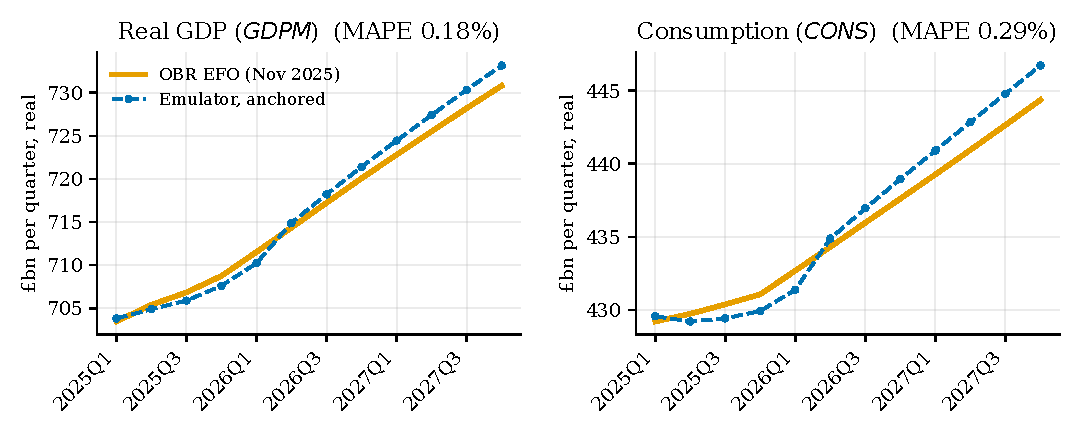
\includegraphics[width=\textwidth]{figures/fig_anchored.pdf}
\caption{Anchored baseline versus the OBR EFO, 2025Q1--2027Q4: current March 2026 EFO anchoring (refreshed 21 July 2026). Real GDP and consumption in \pounds bn per quarter (chained volumes). The anchored fit is a by-construction invariant (Section~\ref{sec:anchoring}), hard-gated in CI at 1 per cent MAPE. On this March-vintage refresh the anchored MAPEs are 0.15 per cent (GDP) and 0.25 per cent (consumption); the adjacent Table~\ref{tab:anchored} (0.18/0.29 per cent) reports the preserved November 2025 study. Generated by \texttt{figures/fig\_anchored.py}.}
\label{fig:anchored}
\end{figure}

\subsection{The free-running model: an honest scorecard}
\label{sec:rawscore}

The true measure of calibration is the raw model with add-factors off. Two flattery traps are removed before scoring. First, \emph{de-seeding}: the solver's data frame is pre-filled with the EFO path, so a quarter whose Gauss--Seidel iteration exits on a stall would otherwise sit near the EFO seed; the scorecard re-solves each period after reseeding every live computed variable from the model's own previous-period value. Second, \emph{passthrough labelling}: a 0.00 per cent error usually does not mean a good forecast---it means the variable was left at the OBR's published value because its equation is dead or exogenous. Only variables the model actually computes measure calibration, and the employment identity ($ETLFS = HWA/AVH$, both passthrough inputs) is flagged as trivial rather than counted as a behavioural win.

The scorecard is now also emitted as structured JSON. Its schema retains all
headline rows but excludes anchored and passthrough quantities from the accuracy
denominator by construction, and states explicitly that the exercise is not a
historical-vintage forecast backtest. This turns the paper's disclosure rule
into a machine-checkable acceptance contract rather than a presentation choice.

Table~\ref{tab:rawscore} presents the scorecard, and Figure~\ref{fig:freerunning} shows what the divergence looks like in levels for three of the computed variables: the free-running model \emph{contracts} while the EFO grows---the raw dynamics lose the OBR's judgement about the recovery path and drift down at roughly 1--2 per cent a year---and household income now sits between \pounds 3bn \emph{above} and \pounds 70bn below the published path (about \pounds 31bn below on average across the horizon), computed directly from \texttt{figures/fig\_free\_running\_data.csv}. That gap was \pounds 33--117bn, about \pounds 71bn on average, before the $OSHH$ ONS level anchor discussed below; the earlier figure is what this paper previously reported. The full 21-variable panel, including every passthrough, is reproduced in Appendix~\ref{app:scorecard}. ``Within band'' collapses per-metric thresholds---rates within 1.0pp, net balances within 1.5 per cent of GDP (the OBR's own convention for scoring a difference of two large gross flows), levels within 10 per cent MAPE.

\begin{table}[ht]
\centering
\caption{Free-running (raw) model versus the OBR March 2026 EFO, 2025Q1--2027Q4}
\label{tab:rawscore}
\small
\begin{tabular}{llrl}
\toprule
Variable & Metric & Error (3yr) & Status \\
\midrule
Real GDP & MAPE & 4.48\% & computed --- fair \\
Consumption & MAPE & 7.49\% & computed --- fair \\
Trade balance & \% of GDP & 0.69\% & computed --- fair \\
Household income & MAPE & 6.27\% & computed --- fair \\
Real household income & MAPE & 6.03\% & computed --- fair \\
Employment & MAPE & 0.00\% & computed --- \emph{trivial identity} \\
Unemployment rate & pp & 1.01 & computed --- poor \\
RPI inflation & pp & 1.71 & computed --- poor \\
Business investment & MAPE & 15.73\% & computed --- poor \\
Current account & \% of GDP & 3.60\% & computed --- \textbf{off} \\
Company profits & MAPE & 63.29\% & computed --- \textbf{off} \\
\midrule
\multicolumn{2}{l}{Investment, exports, imports, employees, avg.\ earnings,} & 0.00\% & passthrough \\
\multicolumn{2}{l}{CPI, CPI inflation, GDP deflator, wages, compensation} & & (held at OBR value) \\
\bottomrule
\end{tabular}

\medskip
\parbox{0.92\textwidth}{\footnotesize \emph{Notes:} De-seeded raw solve, add-factors off, March 2026 EFO vintage; reproduced by \texttt{python -m obr\_macro.calibration\_score} and, for the first two rows and household income, from \texttt{figures/fig\_free\_running\_data.csv} directly. Of 21 headline variables, 11 are computed and 10 are passthroughs; of the 11 computed, 6 land within band (55\%)---real GDP, consumption, both household-income series, the trade balance, and the trivial employment identity. The real-GDP row is not independent of the consumption row: 98--99 per cent of the GDP error is the consumption error (see the anchored discussion above). Bands: rates $<$1.0pp, net balances $<$1.5\% of GDP, levels $<$10\% MAPE. Earlier versions of this table reported 5.70/9.45 per cent for GDP/consumption, 14.76 and 14.48 per cent for the income series and 54.57 per cent for company profits, with 4 of 11 within band; those figures predate the $OSHH$ ONS level anchor and overstated the error. The current account moved the other way, from 2.76 to 3.60 per cent of GDP, because the March EFO revised the current-account path while the $NIPD$ overseas normalisers stayed at their old unpublished levels. Source: \texttt{docs/calibration\_scorecard.md}, generated by \texttt{obr\_macro/calibration\_score.py}.}
\end{table}

\begin{figure}[ht]
\centering
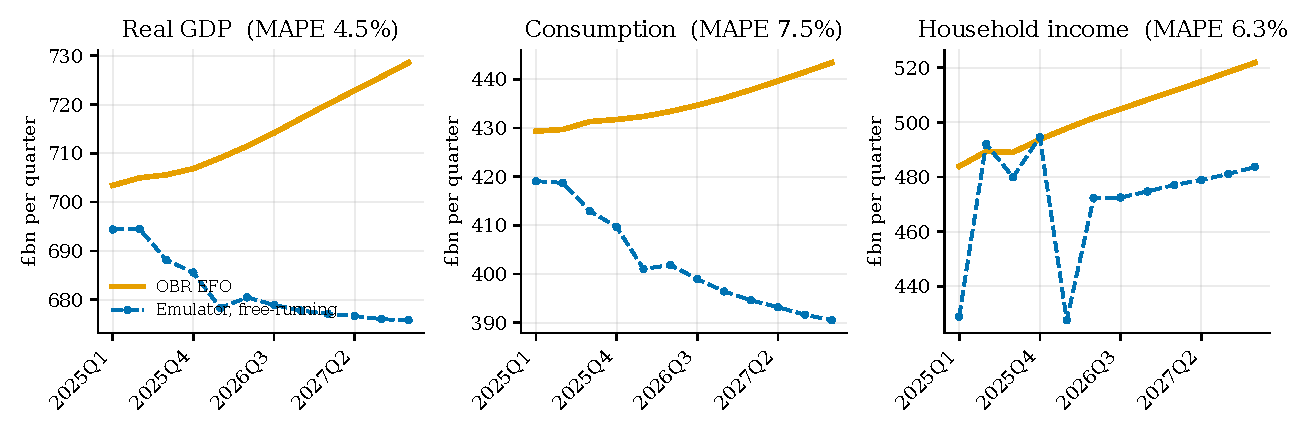
\includegraphics[width=\textwidth]{figures/fig_free_running.pdf}
\caption{Free-running (raw, de-seeded, add-factors off) model versus the OBR EFO, 2025Q1--2027Q4, \pounds bn per quarter, on the current March 2026 anchoring. The panel MAPEs --- 4.48 per cent (GDP), 7.49 per cent (consumption), 6.27 per cent (household income) --- are recomputed here from \texttt{figures/fig\_free\_running\_data.csv} and agree with Table~\ref{tab:rawscore}. The honest divergence: without the OBR's judgement terms the model drifts below the published path for GDP and consumption. Household income no longer inherits the full unpublished $OSHH$ constant gap, which the ONS level anchor closed; the GDP and consumption panels are near-duplicates of each other by construction, since consumption carries essentially the whole GDP error. Generated by \texttt{figures/fig\_free\_running.py}.}
\label{fig:freerunning}
\end{figure}

Three residual errors deserve explanation because they are \emph{floors}, not bugs. The company-profits error (63.3 per cent) traces to households' operating surplus: the published equation $OSHH = 12874 + 0.85\,IROO - DIPHH^{mf}$ evaluates to roughly \pounds 38bn against the OBR databank's roughly \pounds 77bn, and the gap lives in the additive base constant and the vintage of the unpublished rent index feeding $IROO$. Because $HHDI$ \emph{adds} $OSHH$ while $FYCPR$ \emph{subtracts} it, one unpublished constant drives error in three scored variables at once. Anchoring $OSHH$ to the ONS level largely closed the income side (household income fell from 14.8 to 6.3 per cent MAPE, real household income from 14.5 to 6.0) but not the profits side, where the residual is still dominated by the unpublished constant. Re-tuning the constant to hit the target would be fitting to the answer, so it is documented and gated against regression instead. Similarly, RPI inflation decays because the unpublished $I7$/$PR$ index history runs out around 2026Q2, and the current-account error is bounded by overseas rate-of-return normalisers the OBR does not publish. These figures are far better than early development versions (business investment 318 per cent, household income $\sim$932 per cent, company profits $\sim$375 per cent), which reflected genuine bugs in the incomes, investment, and financial-account blocks that were found and fixed; what remains is bounded by unpublished inputs.

\subsection{Held-add-factor forecast}

Between the two extremes sits the forecasting configuration (Section~\ref{sec:anchoring}): add-factors fitted over 2024Q1--2025Q4, held constant, projected over 2026Q1--2027Q4. Recomputed on the March 2026 vintage, real GDP comes in at 0.37 per cent MAPE, consumption 0.33 per cent, unemployment 0.69pp, the trade balance 0.25 and the current account 1.36 per cent of GDP---all within band---while business investment (15.11 per cent) and company profits (12.40 per cent) sit over band: 8 of 16 headline variables are computed and 6 of those land within band. Earlier versions of this paper reported 2.2 per cent for GDP, 3.6 for consumption, $\sim$18 for business investment, $\sim$47 for profits and $\sim$12 for household income, with 10 of 16 computed; those figures predate both the $OSHH$ anchor and \texttt{\_PUBLISHED\_LEVEL\_ANCHORS}.

Three caveats govern how much of that improvement is real, and the last is the most important. The forecast is initialised at the EFO values it is scored against (a neutral jump-off scores worse, and business investment then fails the band); the add-factor base window extends into quarters that are themselves OBR forecast rather than outturn, so the held add-factors partly encode ``agree with the OBR''; and \textbf{household income and real household income are no longer forecast at all}. \texttt{\_PUBLISHED\_LEVEL\_ANCHORS} makes $HHDI$ and $RHHDI$ exogenous, so they are held at their EFO values and score exactly 0.00 per cent by construction --- they have left the computed set rather than improved within it, which is also why the computed count falls from 16 to 8. Any reading of the household-income line as forecast accuracy would be reading a variable with no equation.
